\documentclass{article}
\usepackage[utf8]{inputenc}
\usepackage{amsmath,amsfonts,amssymb,amsthm,mathtools}
\usepackage{parskip}
\usepackage{color}
\usepackage{booktabs}
\usepackage{hyperref}

\newtheorem{exercise}{Exercise}
\newtheorem{answer}{Answer}

\newcommand{\dd}[2][]{\frac{\partial #1}{\partial #2}}
\newcommand{\dt}[2][]{\frac{d #1}{d #2}}
\newcommand{\dL}{\dt[{\L}]}
\newcommand{\dLi}{\dt[{\Li}]}
\newcommand{\dLmb}{\dt[{\Lmb}]}
\newcommand{\dLfb}{\dt[{\Lfb}]}
\newcommand{\yh}{\hat{y}}

\newcommand{\bracket}[3]{\left#1 #3 \right#2}
\newcommand{\sqb}{\bracket{[}{]}}
\newcommand{\ab}{\bracket{\langle}{\rangle}}
\renewcommand{\b}{\bracket{(}{)}}
\newcommand{\abs}{\bracket{\lvert}{\rvert}}

\newcommand{\0}{\mathbf{0}}
\newcommand{\x}{\mathbf{x}}
\newcommand{\y}{\mathbf{y}}
\newcommand{\f}{\mathbf{f}}
\newcommand{\h}{\mathbf{h}}
\newcommand{\g}{\mathbf{g}}
\newcommand{\mom}{\mathbf{v}}
\newcommand{\F}{\mathbf{F}}
\newcommand{\gfb}{\g_\text{fb}}
\newcommand{\gmb}{\g_\text{mb}}
\newcommand{\gmbt}{\g_{\text{mb}; t}}
\newcommand{\gsmbt}{g_{\text{mb}; t}}
\newcommand{\gsfb}{g_\text{fb}}
\newcommand{\gsmb}{g_\text{mb}}
\newcommand{\gsd}{\g_\text{sd}}
\newcommand{\vh}{\hat{v}}
\newcommand{\mh}{\hat{m}}
\newcommand{\gh}{\mathbf{\hat{g}}}
\newcommand{\gb}{\mathbf{\ab{g}}}
\newcommand{\gssqb}{\ab{g^2}}
\newcommand{\gsb}{\ab{g}}
\newcommand{\bv}{\mathbf{b}}
\newcommand{\ov}{\mathbf{o}}
\renewcommand{\a}{\mathbf{a}}
\newcommand{\X}{\mathbf{X}}
\newcommand{\W}{\mathbf{W}}
\newcommand{\I}{\mathbf{I}}
\renewcommand{\P}{\operatorname{P}\b}

\newcommand{\w}{\mathbf{w}}
\newcommand{\wo}{\w^*}

\renewcommand{\L}{\mathcal{L}}
\newcommand{\Li}{\L_i}
\newcommand{\Lmb}{\L_\text{mb}}
\newcommand{\Lfb}{\L_\text{fb}}
\newcommand{\E}{\operatorname{E}\sqb}
\newcommand{\Var}{\operatorname{Var}\sqb}

\newcommand{\logits}{\ell}
\newcommand{\vlogits}{\boldsymbol{\logits}}
\newcommand{\softmax}{\operatorname{softmax}}
\newcommand{\linear}{\operatorname{linear}}
\newcommand{\relu}{\operatorname{relu}}
\newcommand{\sqerr}{\operatorname{sqerr}}

\newcommand{\func}{\operatorname{func}}
\newcommand{\funcback}{\operatorname{func{.}backward}}
\newcommand{\funcjac}{\operatorname{func{.}jacobian}}
\newcommand{\inputs}{\operatorname{inputs}}
\newcommand{\outputs}{\operatorname{outputs}}

\newcommand{\linearback}{\operatorname{linear{.}backward}}
\newcommand{\reluback}{\operatorname{relu{.}backward}}
\newcommand{\sqerrback}{\operatorname{sqerr{.}backward}}

\newcommand{\linearjac}{\operatorname{linear{.}jacobian}}
\newcommand{\relujac}{\operatorname{relu{.}jacobian}}

\newcommand{\iinmb}{{i \text{ in mb}}}
\newcommand{\mbsize}{M}
\newcommand{\mbavg}{\tfrac{1}{\mbsize} \sum_{\mathclap{\iinmb}}}

\newcommand{\iinfb}{{i \text{ in fb}}}
\newcommand{\fbsize}{N}
\newcommand{\fbavg}{\tfrac{1}{\fbsize} \sum_{i=1}^{\fbsize}}
\newcommand{\lrtrad}{\eta_\text{trad}}
\newcommand{\lravg}{\eta_\text{avg}}

\title{EMAT31530, Part 7: How to train your NN}
\author{Laurence Aitchison}
\date{}

\begin{document}

\maketitle

I advise that you take a look at the iPython notebook for this week first, as it discusses overfitting in the simpler setting of linear models.  We take the next step, by discussing Here, we discuss overfitting in the more complex setting of neural networks and how to mitigate overfitting in these models.

\section{Overfitting is not catastrophic in NNs}

In the 1990's, neural networks were largely ignored: only a few people like Yann LeCun were still working on them.
One of the reasons was the following reasoning:
\begin{itemize}
  \item Neural networks have loads (and loads) of parameters.
  \item Models with loads of parameters tend to overfit.
  \item So neural networks should overfit really badly.
\end{itemize}
Surprisingly, it turns out that overfitting is only a very minor issue in NNs.
Specifically, if you just do the naive thing do SGD with the cross-entropy loss for classification or the sqaured error loss for regression, and you'll get pretty darn good result.
You definitely won't get anything like the extreme predictions that sometimes happen in a linear model.

\newpage
\section{Training dynamics}

\includegraphics[width=\textwidth]{smooth_interp.pdf}

Here, I fitted a three-layer network with width 100 hidden layer, to 20 datapoints drawn from $\sin(x) + \text{noise}$.

There are two features to notice here.
\begin{itemize}
  \item Earlier in training (lighter lines) the function is smooth, it gradually gets more "details" as training progresses.
  \item Later in training (darker lines), the line basically goes through all the datapoints. Strictly speaking, this is overfitting, as its fitting the noise rather than the ``real underlying'' sin function (especially see the ``dip'' about $x=-1$.  But actually, this is a pretty darn reasonable prediction, e.g.\ nothing has blown up.
\end{itemize}
Finally, once the network has found a line that goes through all the datapoints, then there are no more gradients, and the weights don't change any more.

\newpage
\section{Adam vs SGD}

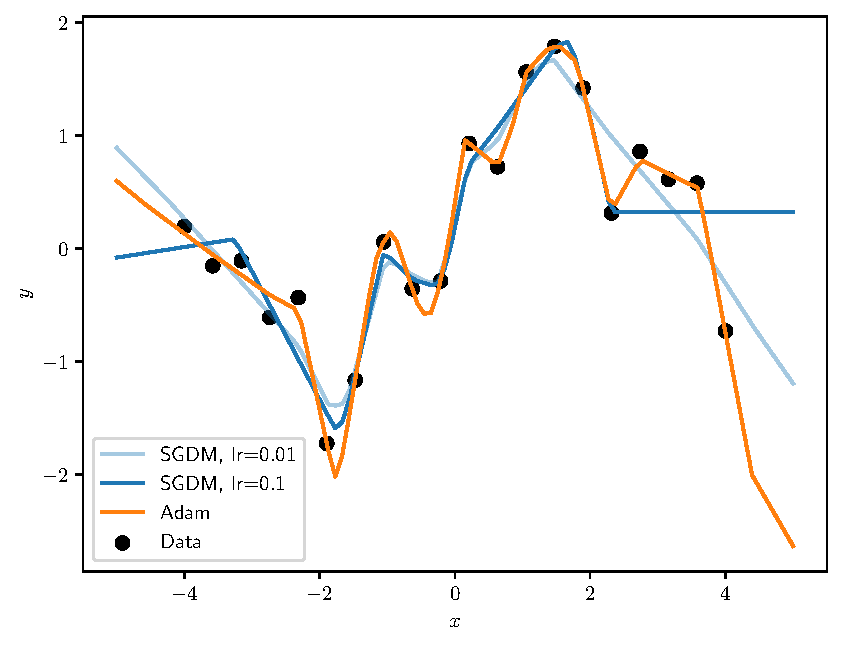
\includegraphics[width=\textwidth]{adam_vs_sgd.pdf}

It seems that:
\begin{itemize}
  \item Adam is better at capturing ``fine details'' than SGD.
  \item Adam tends to overfit more than SGD.
\end{itemize}
These are really just two sides of the same coin: overfitting \textit{is} capturing the fine details (specifically, fine details in the noise).

So which is best Adam or SGD?  Depends on whether you care about mitigating overfitting or capturing fine-details.
\begin{itemize}
  \item SGD tends to be better for ConvNets (which we'll look at next week) for image recognition, as it mitigates overfitting.
  \item Adam tends to be better for transformers (which we'll look at in a couple of weeks), RL where capturing fine-details seems to be mroe relevant.
\end{itemize}

\newpage
\section{Warm up}

Why does SGD tend to avoid capturing fine-details?  Well, once the function is close-enough, the gradients are small, so SGD makes little progress.
How can we improve?  We can increase the gradients after 

\newpage
\section{Minibatch noise}

\newpage
\section{Weight decay}
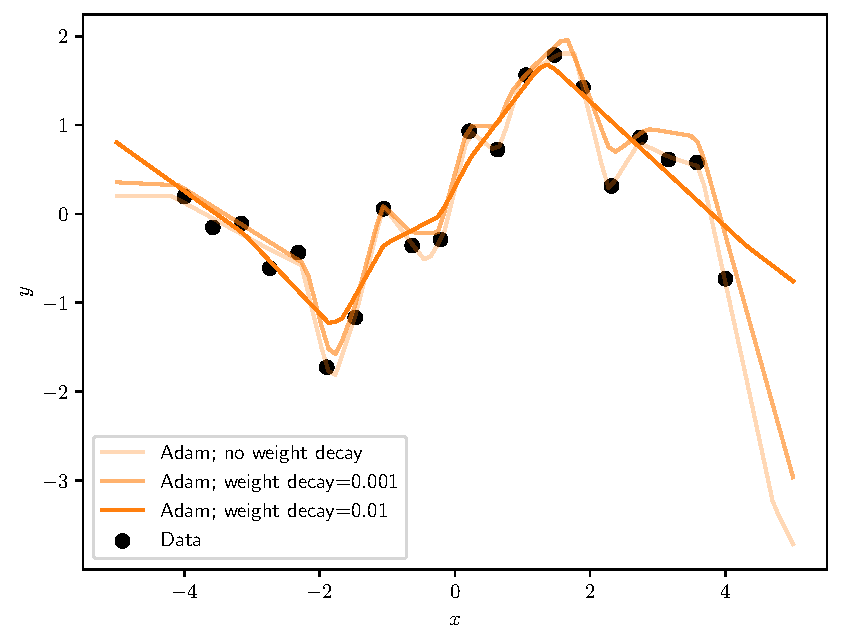
\includegraphics[width=\textwidth]{weight_decay.pdf}

\newpage
\subsection{``Decoupled'' weight decay}
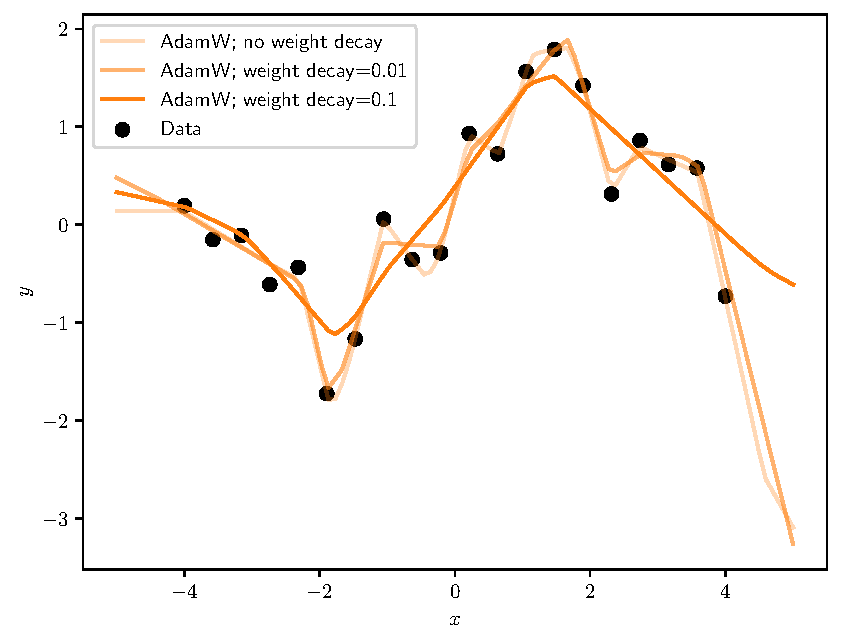
\includegraphics[width=\textwidth]{decoupled_weight_decay.pdf}

\newpage
\section{Dropout}
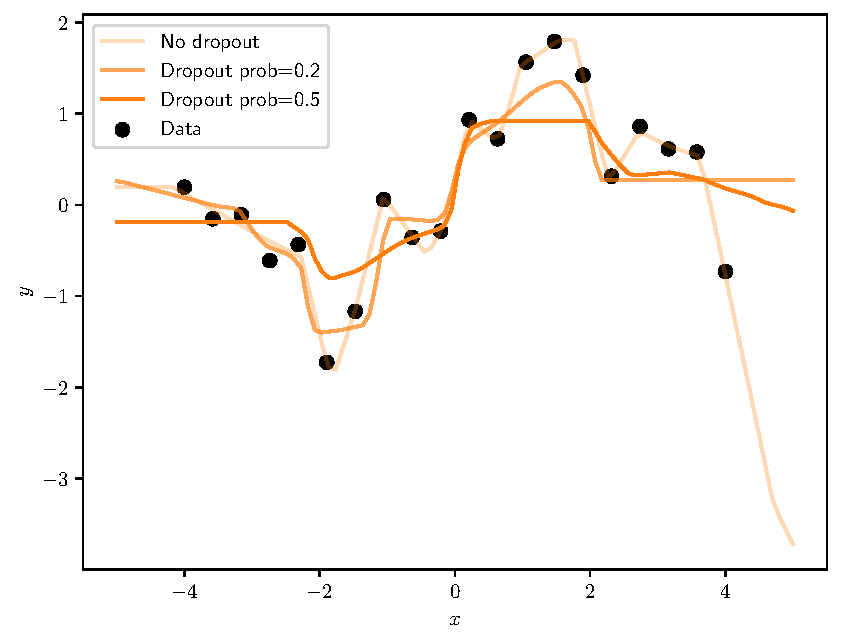
\includegraphics[width=\textwidth]{dropout.pdf}

\section{Exercises}

\begin{exercise}
\end{exercise}

\begin{answer}
\end{answer}


\end{document}

